% $Id: typing.tex,v 1.12 2009-05-12 18:02:35 pessaux Exp $

The type-checking pass performs in fact several important tasks. It
obviously infer the type of each expression and construct, but it also
performs inheritance resolution, compute dependencies on methods of
{\tt Self} (def and decl-dependencies), ensure that the species are
well-formed and sort the methods in order they are properly ordered.
Once the type-checking pass is ended, a processed species gets in
normal form, i.e. with all its methods present once, inherited and
defined ones having been consistently put together.

\label{cool-incremental-nf}
This especially means that at each inheritance step, any species
issued by the type-checker has all its methods: the inheritance
disappears from the species structure. Obviously, the still have means
to know about the inheritance history somewhere, but all the methods,
inherited, defined, declared are always all together in a species in
normal form.

In other words, considering only the bunch of methods a species has,
there is no difference between a species having them via inheritance
and a species having them in its own current body with no
inheritance.

This point is especially important since it allows to inductively be
sure that if one inherits of a species, then in just one shot we know
which methods we have inherited: there is no need to walk again along
all the inheritance steps. Then, we can says that we inductively build
the normal form of species all along the inheritance tree. This point
allows faster searches and prevent from having information
disseminated in several place which would be more difficult to
maintain.

In fact, the scoping pass already used a similar way to proceed,
keeping for each species the list of all the methods it had, either in
its own body or by arbitrary inheritance.

\label{becoming-of-typing-output}
The output of the typing pass is a {\tt Infer.please\_compile\_me}
structure in which we have both the AST of the definitions and
information computed during typing. This structure will then be passed
to the ``abstraction'' stuff (directory {\tt src/commoncodegen}) to
compute extra dependency information and group all the dependencies
together and factorise some computations required by code generation
(more especially, what to lambda-lift and to instanciate). This
``abstraction'' pass is called before calling the code generation by
each code generator back-end (in fact, called by each target code
generator).

\medskip
We will now examine various points of this typing pass.




\section{Type inference}
\subsection{Where to record type information in the AST ?}
Type inference is the process of guessing the type of each expression,
each definition of the source code. In fact, in \focalize, types are
partly inferred, partly given by the programmer. Signatures are a way
to make types explicit by giving annotations. However, at each node of
the AST, types must be infer-ed to finally label the node. In effect,
the first output of the type-checking pass it a ``typed AST'',
i.e. the initial AST with each node now having its type recorded in
the node itself.

As defined in the source file {\tt basement/parsetree.mli}, an AST
node is a generic data-structure containing a specific description:

{\footnotesize
\begin{lstlisting}[language=MyOCaml, title=Generic AST node]
type 'a ast = {
   (** The location in the source of the AST node. *)
   ast_loc : Location.t;
   (** The description of the node. *)
   ast_desc : 'a;
   (** The support for documentation. *)
   ast_doc : documentation;
   (** The type of the node. *)
   mutable ast_type : ast_node_type_information;
}
\end{lstlisting}
}
Hence, a node containing an expression (hence of type
{\tt Parsetree.expr}) will be built by something like:

{\footnotesize
\begin{lstlisting}[language=MyOCaml, title=An ``expression'' AST node]
type expr_desc =
  | E_self
  | E_const of constant
  | E_fun of vname list * expr
  | ...

type expr = expr_desc ast
\end{lstlisting}
}

In the generic data-structure of the node, the field
{\tt ast\_type} is used to record the type inferred for this
node. Since we want to keep the same AST structure all along the
compilation process, we use a mutable field for the type because
initially, after lexing/parsing and scoping, the type is not yet
known. So, the type-checking pass will modify the value contained in
this field for each node of the AST.

According to the source file {\tt basement/parsetree.mli}, values for
this field can be:

{\footnotesize
\begin{lstlisting}[language=MyOCaml, title=An ``expression'' AST node]
type ast_node_type_information =
   | ANTI_non_relevant   (** The node has no meaningful type information.
			     However, it was processed by the type-checker. *)
   | ANTI_none      (** The node was not yet processed by the type-checker.
		        Clearly, after the type-checking pass, no AST node
			should remain with this tag in the [ast_type] field of
			the node ! *)
   | ANTI_type of Types.type_simple  (** The type information is a type. Mostly
					 used to label expressions. *)
   | ANTI_scheme of Types.type_scheme (** The type information is a type scheme.
					  Mostly used to label definitions. *)
\end{lstlisting}
}

Before type-checking is done, all the node of the AST have their
{\tt ast\_type} field worthing {\tt ANTI\_none}. Once the
type-checking pass is done, no AST node should remain with this
tag. If some do, then is must be considered as a bug (node forgotten
during processing) of the compiler. At least, when a node does not
require a type information (for instance, the AST node of a {\tt open}
directive), it must however be traversed by the type-checker and must
be updated with the {\tt ANTI\_non\_relevant} value.



\subsection{Types and type schemes}
\index{type!scheme}
\label{type-scheme}
Like in regular ML-like type-checkers, expressions are assigned
``types'' although definitions are assigned ``type schemes''. The
difference is due to the ability for definitions to be polymorphic and
to be instantiated differently at each usage occurrence. In effect, an
expression exists in only one point. So it has one {\bf type}, that's
all. A definition leads to a ``template'' of types, where polymorphic
type variables car be instantiated as wished each time the identifier
bound by the definition is used. For this reason, a definition is
bound to a ``model'' of types, a ``family'' of type, that is usually
called a {\bf type scheme}.

Then a type scheme is in fact a list of polymorphic type variables and
a body that is a type expression. For instance, the ML-like type scheme
(possibly bound to a {\tt List.map} function)
{\tt ('a -> 'b) -> 'a list -> 'b list} will be represented by the list
of it's 2 type variables {\tt 'a} and {\tt 'b} and its body that is
the expression {\tt ('a -> 'b) -> 'a list -> 'b list}. In fact, in a
type scheme all the polymorphic type variables are {\bf implicitly
quantified universally}. The ``implicitly'' is the reason why it is
so difficult for the programmer to really see the difference between a
type and a type scheme. For the above type scheme, we should be more
explicit and better write:

$\forall$ {\tt 'a, 'b . ('a -> 'b) -> 'a list -> 'b\ list}

If we now have a look at the following expression:
{\tt List.map (fun x -> x + 1)}, then the expression (i.e. the
identifier node) {\tt List.map} will have the {\bf type}
{\tt ('t -> 'u) -> 't list -> 'u list} (in which we intentionally
changed the names of the types variables to show that they are {\bf not
the same} that those of the type scheme). This type expression
contains 2 variables {\tt 't} and {\tt 'u} that will be unified during
the type-checking of the whole application expression (unified with
{\tt int} in the current example).

\medskip
In \focalize, type schemes are compound of the list of the polymorphic
type variables that are its parameters and the type expression that is
its body:
{\footnotesize
\begin{lstlisting}[language=MyOCaml, title=An ``expression'' AST node]
type type_scheme = {
  ts_vars : type_variable list ;          (** Parameters in the scheme. *)
  ts_body : type_simple    (** Body of the scheme where generalized types
                               have a level equal to [generic_level]. *)
}
\end{lstlisting}
}



\subsection{Working ``in place'' with substitutions}
The type-checking algorithm of ML-like languages is often stated using
the notion of MGU and using substitutions. In \focalize, the effective
inference algorithm uses techniques more efficient in practice than
regular substitutions to manually apply and combine on the type
terms. Instead, we work ``in place'', by taking benefits of sharing
between type sub-terms to simulate the substitutions by direct
physical modifications inside the terms.

\medskip
The full description of this technique is outside the scope of the
present document, but a clear and efficient explanation can be found
in ``Le langage Caml'' written by Pierre Weis and Xavier Leroy.

\medskip
The idea is to represent the types by terms that can be physically
shared, with type variables that can be directly assign a
value. Hence, as described in the source file {\tt basement/type.ml},
our type algebra is:

{\footnotesize
\begin{lstlisting}[language=MyOCaml, title=An ``expression'' AST node]
type type_simple =
  | ST_var of type_variable                   (** Type variable. *)
  | ST_arrow of (type_simple * type_simple)   (** Functional type. *)
  | ST_tuple of type_simple list              (** Tuple type. *)
  | ST_sum_arguments of type_simple list      (** Type of sum type value
                                                  constructor's arguments. To
                                                  prevent them from being
                                                  confused with tuples. *)
  | ST_construct of
      (** Type constructor, possibly with arguments. Encompass the types
          related to records and sums. Any value of these types are typed as
          a [ST_construct] whose name is the name of the record (or sum)
          type. *)
      (type_name * type_simple list)
  | ST_self_rep     (** Carrier type of the currently analysed species. *)
  | ST_species_rep of
      (** Carrier type of a collection hosted in the specified module. *)
      (fname * collection_name)


and type_variable = {
  (** Binding level of the type. *)
  mutable tv_level : int ;
  (** Value of the type variable. *)
  mutable tv_value : type_variable_value
}


and type_variable_value =
  | TVV_unknown
  | TVV_known of type_simple
\end{lstlisting}
}

The algebra describes the built-in type constructors and more
interestingly for our explanation, the {\bf type variables}. We can
see that in the type algebra, all the variables look pretty
structurally the same: the constructor {\tt ST\_var} and a
{\tt type\_variable} containing a few information. Hence, for instance
2 variables whose value are unknown will look exactly the same. To
make the difference, we must consider physical equality. Hence, if 2
variables are physically equal, ``they are {\bf the} same''
variable(s?), otherwise they are really different. The aim of this
mechanism is to share the same physical data to represent all the
occurrences of a variable in a term, so that when we want to assign it
a value, we just need to modify it in place and all the shared
occurrences will be updated for free.

A type variable is initially an unknown of the unification equation
induced by the type-checking process. Hence it starts with its field
{\tt tv\_value} worthing {\tt TVV\_unknown}. If during unification, a
variable needs to be assigned a value (i.e. a constraint was found on
this variable), then its {\tt tv\_value} that is mutable will be
assigned {\tt TVV\_known} ``of something''. This ``something'' is
itself a type and this allows indeed to instantiate a type variable by
a type expression.

Obviously, this mechanism to represent instantiations will create
``strings'' of links between variables and their effective value. To
be sure that the value of a variable is know ``equal to something'' or
really unknown, we must use a mechanism that returns the canonical
representation of a type. For instance, let's imagine that in our
inference problem, we arrived to have 4 variables $\alpha$, $\beta$,
$\gamma$ and $\delta$, with $\alpha = \beta$, $\beta = {\tt int}$,
$\delta = \gamma$ and $\gamma = \beta$. Hence, we have the following
picture:

\noindent
\begin{math}
\begin{array}{ccccc}
\alpha & \rightarrow & \beta & \rightarrow & {\tt int} \\
       &             & \uparrow & & \\
\delta & \rightarrow & \gamma & &
\end{array}
\end{math}

\noindent representing the system: where
{\footnotesize\lstinline!'a = ST_var (TVV_known (...))!} where
{\footnotesize\lstinline!...!} represents {\tt 'b} and has the
structure
{\footnotesize\lstinline!ST_var (TVV_known (ST_construct (``int'', [])))!}.
We have the same kind of thing for $\delta$ and $\gamma$, with
$\gamma$ worthing
{\footnotesize\lstinline!TVV_known (...)!} with
{\footnotesize\lstinline!...!} representing the structure of $\beta$.
In fact, despite all the variables we see above, all are equal and are
instantiated by {\tt int}. This means than must not trust the first
value constructor seen for a type to know what it is equal to. One
must ``follow'' the links.

Moreover, to avoid the loss of efficiency induced by walking each
time along these ``strings'' of links, the operation of getting the
canonical representation of a type will use the ``path compression''
operation in order to suppress indirections a soon as they are
encountered a first time.

The operation returning the canonical representation is the guardian
of the correct structure of the types. {\bf Any operation working /
relying / walking on the type structure must call this operation to be
sure that the structural view of the type is has is really the
canonical view of the type}. This operation called {\tt repr} is
located in the {\tt basement/types.ml} source file of the
compiler. The presence of such a strong invariant is the reason why
the types are exported as {\bf abstract}. This ensures that outside
the module manipulating the type algebra, nobody will forget to get
the canonical representation of a type.

Basically, this function receives a type. If this type is not a
variable, then it returns it directly. This means that the type
constructor is already known to be something else than a variable for
which we should investigate further. On the other side, if the
received type is a variable whose ``value'' (i.e. field
{\tt tv\_value} is ``known to be equal to something'' (i.e. is
{\tt TVV\_known (...)}, then we will ask to get the canonical
representation of this ``something''. This is typically a recursive
call on this ``something''. This way, if this ``something'' is itself
a variable ``known to be equal to something else'', then we will
inductively know each step of indirection. So, once we get our
canonical representation of our ``something'', {\bf this is} in fact
the canonical representation of our type, since it was a variable
``known to be equal to {\bf this} something''. By the way, before
returning, since now we know that the variable is in fact ``pointing''
onto a type (i.e. is not anymore a variable, was instantiated), we
take benefit to cut the string of indirections by directly
establishing a link between the variable and the canonical
representation we obtained. Hence, next time we will access this
variable via a type sub-term shared somewhere else, we won't have
anymore to walk along the whole ``string'' of links to know the
variable's value. Then, the {\tt repr} function simply looks like:

{\footnotesize
\begin{lstlisting}[language=MyOCaml,
                   title=Getting the canonical representation of a type]
let rec repr = function
  | ST_var ({ tv_value = TVV_known ty1 } as var) ->
      let val_of_ty1 = repr ty1 in
      var.tv_value <- TVV_known val_of_ty1 ;
      val_of_ty1
  | ty -> ty
\end{lstlisting}
}


\subsection{Unification}
The computation of the most general type of an expression, called type
inference, strongly rely on unification of type terms. We will say
that 2 terms $\tau_1$ and $\tau_2$ can be {\em unified} if there exists
a substitution $\phi$ so that $\phi(\tau_1) = \phi (\tau_2)$. The
substitution $\phi$ is then called {\em unifier}.
\index{unifier} of the terms $\tau_1$ and $\tau_2$. Hence, two terms
can be unified if it is possible to instantiate all or part of their
variables by a same substitution, so that they become structurally
equal.

Based on the representation of our types, since the unification tends
to return a substitution to apply on the 2 unified types in order to
make them equal, instead of getting this substitution to later apply
it to each type (and combine this substitution with the other
substitutions the types may be subject to), we will directly make the
type terms equal by instantiating their type variables. The
``instanciation'' is then made in place, by changing in place the
mutable field {\tt tv\_value} of the unknown variables from
{\tt TVV\_unknown} to {\tt TVV\_known} ``of'' the type required to
have equality.

This is especially fast since all the occurrences of a variable share
the same physical location. Hence, changing the value of the field
{\tt tv\_value} at this location is equivalent to simultaneously
instantiate all the occurrences of this variable (past and future) in
type terms.

Hence, ideally unification doesn't return any result and makes the 2
unified type equal by side effect or fails because there exist no
unifier for the 2 types. And then, in the type-checking algorithm,
instead of using one of the type on which we apply its related
substitution, we can directly use any one of the 2 types once unified
since they are now equal.

In fact, in our case this is not completely the case since we have an
additional problem that forces us to return a type. This is due to
the fact that when unifying a type and {\tt Self}, \focalize's rules
require to have {\tt Self} as unification result rather than any of
one the two types. This is a problem when the unification used the
known representation of {\tt Self} to achieve finding the mgu. In
effect, in this case, one of the 2 type is {\tt Self} and this other
is a type expression that is compatible with {\tt Self}'s
representation. And in this fact, choosing any of the 2 types as result
is wrong: the result must always chose (prefer) {\tt Self}. Hence our
unification routine returns the preferred unifier in addition to make
the physical modifications in place when required. We then have a
unification function described in the compiler's source file
{\tt basement/types.ml} looking like (explanations follow):

\label{unify-source-code}
{\footnotesize
\begin{lstlisting}[language=MyOCaml,numbers=left, firstnumber=0,
                   title=The unification algorithm]
let unify ~loc ~self_manifest type1 type2 =
  let rec rec_unify ty1 ty2 =
    let ty1 = repr ty1 in
    let ty2 = repr ty2 in
    if ty1 == ty2 then ty1 else
    match (ty1, ty2) with
     | (ST_var var, _) ->
         (* BE CAREFUL: [occur_check] performs the setting of decl-dependencies
            on the carrier ! In effect, if [ty2] involved Self then we have a
            dependency on the carrier and that must be taken into account !
            The interest to make [occur_check] doing this work is that it
            walk all along the type so it's a good idea to take benefit of this
            walk to avoid one more walk. *)
         occur_check ~loc var ty2 ;
         lowerize_levels var.tv_level ty2 ;
         var.tv_value <- TVV_known ty2 ;
         ty2
     | (_, ST_var var) ->
         (* BE CAREFUL: Same remark than above for [occur_check]. *)
         occur_check ~loc var ty1 ;
         lowerize_levels var.tv_level ty1 ;
         var.tv_value <- TVV_known ty1 ;
         ty1
     | ((ST_arrow (arg1, res1)), (ST_arrow (arg2, res2))) ->
         let arg3 = rec_unify arg1 arg2 in
         let res3 = rec_unify res1 res2 in
         ST_arrow (arg3, res3)
     | ((ST_sum_arguments tys1), (ST_sum_arguments tys2)) ->
         let tys3 =
           (try List.map2 rec_unify tys1 tys2 with
           | Invalid_argument "List.map2" ->
               (* In fact, that's an arity mismatch on the types. There is a
                  strange case appearing when using a sum type constructor that
                  requires arguments without arguments. The type of the
                  constructor's arguments is an ampty list. Then the conflict is
                  reported as "Types and ... are not compatible". Hence one of
                  the type is printed as nothing (c.f. bub report #180).
                  In this case, we generate a special error message. *)
               if (List.length tys1) = 0 || (List.length tys2) = 0 then
                 raise (Arity_mismatch_unexpected_args (loc))
               else raise (Conflict (ty1, ty2, loc))) in
         ST_sum_arguments tys3
     | ((ST_sum_arguments _), (ST_tuple _))
     | ((ST_tuple _), (ST_sum_arguments _)) ->
         (* Special cases to handle confusion between sum type value
            constructor's that take SEVERAL arguments and not 1 argument that
            is a tuple. *)
         raise (Arity_mismatch_unexpected_args (loc))
     | ((ST_tuple tys1), (ST_tuple tys2)) ->
         let tys3 =
           (try List.map2 rec_unify tys1 tys2 with
           | Invalid_argument "List.map2" ->
               (* In fact, that's an arity mismatch on the tuple. *)
               raise (Conflict (ty1, ty2, loc))) in
         ST_tuple tys3
     | (ST_construct (name, args), ST_construct (name', args')) ->
         (if name <> name' then raise (Conflict (ty1, ty2, loc))) ;
         let args'' =
           (try List.map2 rec_unify args args' with
           | Invalid_argument "List.map2" ->
               (* In fact, that's an arity mismatch. *)
               raise
                 (Arity_mismatch
                    (name, (List.length args), (List.length args'), loc))) in
         ST_construct (name, args'')
     | (ST_self_rep, ST_self_rep) ->
         (begin
         (* Trivial, but anyway, proceed as everywhere else. *)
         set_decl_dep_on_rep () ;
         ST_self_rep
         end)
     | (ST_self_rep, _) ->
         (begin
         match self_manifest with
          | None -> raise (Conflict (ty1, ty2, loc))
          | Some self_is_that ->
              ignore (rec_unify self_is_that ty2) ;
              set_def_dep_on_rep () ;
              (* Always prefer Self ! *)
              ST_self_rep
         end)
     | (_, ST_self_rep) ->
         (begin
         match self_manifest with
          | None -> raise (Conflict (ty1, ty2, loc))
          | Some self_is_that ->
              ignore (rec_unify self_is_that ty1) ;
              set_def_dep_on_rep () ;
              (* Always prefer Self ! *)
              ST_self_rep
         end)
     | ((ST_species_rep c1), (ST_species_rep c2)) ->
         if c1 = c2 then ty1 else raise (Conflict (ty1, ty2, loc))
     | (_, _) -> raise (Conflict (ty1, ty2, loc)) in
  (* ****************** *)
  (* Now, let's work... *)
  rec_unify type1 type2
;;
\end{lstlisting}
}

First of all, we see that as previously said, since we intend to work
on the structure of the types, we start by computing their canonical
representation by calling {\tt repr} (lines 2 and 3).

If the 2 types are already the same (physically, note the usage of
{\tt ==} and not {\tt =}), then there is nothing more to to and we can
return any one of the 2 types as unifier. We can really return any one
since they are really equal and the problem of preferring {\tt Self}
doesn't apply here: either the 2 types are both {\tt Self} or they are
both something else.

Then the algorithm considers all the cases of two types. When one is a
variable (lines 6 and 17), we assign to the variable the other type
hence telling that the variable is not anymore unknown (lines 15 and
21).

Before assigning the variable, we perform an ``occur check''
\index{occur check}
(lines 13 and 19). This ensures that the variable we assign doesn't
appear in the type is it assigned. This is to prevent types from being
cyclic. In effect, if we try to unify $\alpha$ with $\alpha
\rightarrow \alpha$, we get in the following situation:

\noindent
\begin{math}
\begin{array}{ccc}
\alpha     & \rightarrow & \alpha \\
 \uparrow  &             & \downarrow  \\
           & \leftarrow &
\end{array}
\end{math}

\noindent with the arrow on the same line than the $\alpha$s
represent the functional type constructor and the arrows below the
link the unification creates between variables and types. Hence, if
the unification falls in this case, an error is raised telling that
the type of the expression leads to cyclic types and that this
expression is rejected. Below is the code of the occur check in which
the line 12 and 13 can be skipped (they will be examined in 
\ref{deps-on-carrier}).

\label{occur-check-source-code}
{\footnotesize
\begin{lstlisting}[language=MyOCaml,numbers=left, firstnumber=0,
                   title=Occur check routine]
let occur_check ~loc var ty =
  let rec test t =
    let t = repr t in
    match t with
     | ST_var var' ->
         if var == var' then raise (Circularity (t, ty, loc))
     | ST_arrow (ty1, ty2) -> test ty1 ; test ty2
     | ST_sum_arguments tys -> List.iter test tys
     | ST_tuple tys -> List.iter test tys
     | ST_construct (_, args) -> List.iter test args
     | ST_species_rep _ -> ()
     | ST_self_rep ->
         (* There is a dependency on the carrier. Note it ! *)
         set_decl_dep_on_rep () in
  test ty
\end{lstlisting}
}

Let's go back to our unification routine. For the moment, the lines 14
and 20 (and the comment lines 7-12) can be forgotten since they will
be explained when we will be dealing with polymorphism.

When unifying with one type being a variable, the returned type is
always the type assigned to the variable (lines 16 and 22). We could
also choose to return the variable but this would be less efficient
since no {\tt repr} is yet applied since we assigned it a value, then
to use this variable as type, one {\tt repr} will immediately be
required. Choosing to return the other type that has been
``{\tt repr}-ed'' we can save one call. This may seems a tiny
advantage, but unification in place is efficient for several tiny
advantages put together ! An this one is part of them.

\medskip
In term of difficulty, we now have the unification of {\tt Self} and a
type. The simplest case (line 65) is the unification of {\tt Self} and
itself. Trivially, the unification succeed. Forget the line 66 for the
moment. There remain 2 symmetric cases: unifying {\tt Self} and another
type that is not {\tt Self} and not a variable (lines 71 and 81).
In these cases, we are in the rules [{\tt Self1}] and [{\tt Self2}] of
Virgile Prevosto's PhD, page 27, definition 9. These are the cases
where, if the structure of the carrier (i.e. of the {\tt representation}
method) is visible then an occurrence of {\tt Self} is allowed to be
unified with a type having a structure compatible with the one given
by the {\tt representation} method.

To be able to make so, in the typing context, we record if the
structure of the carrier is known of not. This information if passed
to the unification function via the parameter
{\tt $\sim$self\_manifest}. This parameter has type
{\tt simple\_type option}. If the value is {\tt None}, this means that
the structure of the carrier is not visible (hence {\tt Self} can only
be unified with {\tt Self}). If the value is {\tt Some ...}, then this
means that we know that the carrier was defined as the type ``...''
(hence unifying {\tt Self} with a type expression compatible with
``...'' must be successful).

So, when unifying {\tt Self} with a type, if {\tt $\sim$self\_manifest}
is {\tt None} we raise an error because the carrier is abstract. If 
{\tt  $\sim$self\_manifest} is {\tt Some (}$\tau${\tt )}, then we must
ensure that $\tau$ can be unified (and if so, the possible side
effects induced by this unification must be done) with the other type
(lines 76 and 96): it is then simply a recursive call. Since if the
unification succeed we want to return {\tt Self} as unifier, we throw
the result an return {\tt ST\_self\_rep}, meaning the type
``{\tt Self}''.

{\bf Attention}: With this mechanism, we directly unify the type that
represents the structure of the carrier. This means that we directly
apply modification in place on it. This especially means that, because
this is not a type scheme but a type, there is a cumulative effect of
all the unifications that are made between {\tt Self} and other
types. Hopefully, this is not a problem since methods are not allowed
to be polymorphic. And {\tt representation}, defining the structure
of {\tt Self} is a method. So it can't be polymorphic. This especially
means that the structure of {\tt Self} will never have remaining
variables that could be instantiated by a unification. Hence, there is
no risk that a unification pollutes the type used as reference for the
structure of {\tt Self} by instantiating a type variable by a type
that would be incompatible for a later unification of this variable by
another type. Sooooo, this means that {\tt $\sim$self\_manifest} is a type
and not a type scheme because we don't have polymorphism on
methods. If we had some, we would need another mechanism to ``prefer
{\tt Self}'' during unification (problem of specialisation,
generalisation, putting the right binding level, and so on\ldots).


\medskip
The other cases of unification are simpler and structural. The
unification can now only be successful if the 2 types have the same
constructor. So we check the types 2 by 2 with each time the same
constructor and if the matching is right, we recurse structurally on
the types structures.

\medskip
Finally remains the all cases where the 2 types do not have the same
constructor (line 93). This leads to a type-checking error by raising
an exception.

\subsection{Polymorphism}
Like introduced in \ref{type-scheme}, type schemes are used to
implement the polymorphism in type inference. They act as ``models''
of types. But the question is how to make such ``models'' and how
extract types from such ``models''. The first point is handled by the
{\tt generalize} function and the second by the {\tt specialize}
function of the source file {\tt basement/types.ml}.

We must start our explanation by introducing the notion of
{\bf binding level}. The aim is to keep trace of type variables
introduced in let-definitions that are deeper than our level. The
binding level counts the number of nested let-definitions. Hence, the
current level must be incremented each {\bf before} every potentially
generalisable definition. This increase will enable the generalisation
once we will go back to a lower level. And it must be decreased at the
end of this definition. To increase the current binding level, the
function {\tt begin\_definition} must be used; to decrease it the
function {\tt end\_definition} must be used.

We said ``potentially generalisable'' definition since all
let-definitions can't be generalised (non-expansivity problem).

There remains a little problem with the level of variables. The higher
the level, the closest is the definition that introduced this type
variable. When a variable is put in contact (i.e. unified) with a type
containing variables with a lower level (i.e. created in outer
let-definitions), hence that may not be generalisable when we will
leave the current definition, we must reflect this onto our variable !
In effect, unification means equality. So if our variable is ``equal''
to a variable than can be generalised, so it must be for our
variable. Hence, when unifying a variable with a type, we must hunt in
this type for variables that have a lower level and if we find some,
we must lower the level of our variable to this found level. That's
what the function {\tt lowerize\_levels} does. And in effect, this
function is called when unifying a type variable with something (lines 
14 and 20 in the {\tt unify} function listed above).


\medskip
So, the generalisation process consists in considering as
generalisable, all the variables having a level strictly greater than
the current binding level. We then search for all the generalisable
variables, and remind them in a list. By the way, we change in place
the level {\tt tv\_level} field) of the found variables by setting a
level meaning ``generalised'' (technically, we choose a value to big,
that there is no chance that anybody nests so many let-definitions to
reach this level). Finally, to build the type scheme, we simply
create a {\tt type\_scheme} structure with the list of found variables
and the type itself as body.

\medskip
Now, taking an instance of a type scheme is done by the function
{\tt specialize} that simply create a fresh type variable for each
generalised variable of the type scheme, then copies the body of the
type scheme, replacing each generalised variable by the corresponding
fresh one.


\subsection{Type inference among other typing things to do}
The type inference we spoke about deals with expressions and
definitions. Hence it is only one part of the analyses performed
during the ``typing pass''. More accurately, it is the first analysis
carried out after the scoping. Each expression of a program must be
type-checked anyway where it appears, in entity parameters, in
methods, in toplevel definitions. Some other constructs of the
\focalize\ language require some other kinds of type-checking: that is
the case of species, collections, collection parameters, inheritance
species expressions. However, during these other kinds of
type-checking, we use the type-checking of expressions to make the
``glue'' ensuring consistency. Rules given in Virgile' PhD in figure
3.2, page 43, section 3.8 are example of this idea (these rules deal
with with species parameters).

\medskip
Aside this notion of type-checking, we also have other analyses to
ensure a program is sound and also to extract the basic shape of a
species by resolving inheritance and late binding. All these things
are performed during the typing pass, the type-checking being the
first step.

\medskip
The typing pass is driven by the source file {\tt typing/infer.ml} and
more especially by the entry point function {\tt
  typecheck\_file}. This function triggers the type-checking of each
phrase of the compilation unit. Be aware that in the source of the
compiler, ``type-check'' is widely overloaded and denotes the process
of inferring type for entities and then ensuring they are well-formed
and building the first pieces of information that will ease the code
generation. In particular, the fact that each species is given a
normal form containing all its methods is handy to recover the methods
of parameters or inheritance species expressions since there is no
need to walk along all the inheritance level (point already mentioned
in the introduction of this chapter, at \ref{cool-incremental-nf}).



\section{Environment and structures for typing pass}
The structure of the environment used during the typing pass has been
presented in \ref{typing-environment} and is coded in {typing/env.ml}.

The only other structure used during this pass is the typing context
that group various information to pass to the functions instead of
having to pass them individually hence preventing from having tons of
arguments for each call. This structure, shown below is local to
the {\tt typing/infer.ml} and passed to each function under the
parameter name {\tt ctx}.

{\footnotesize
\begin{lstlisting}[language=MyOCaml, title=Typing context]
type typing_context = {
  (** The name of the currently analysed compilation unit (i.e. the name
      of the file without extension and not capitalized). *)
  current_unit : Types.fname ;
  (** The name of the current species if relevant. *)
  current_species : Parsetree.qualified_species option ;
  (** Optional type Self is known to be equal to. *)
  self_manifest : Types.type_simple option ;
  (** Mapping between 'variables [vname]s and the [simple_type] they are
      bound to. Used when creating a polymorphic type definition. *)
  tyvars_mapping : (Parsetree.vname * Types.type_simple) list
}
\end{lstlisting}
}




\section{Typing a species definition}
The process of typing a species will be now examined step by step by
step. This is done by typing its parameters, resolving inheritance,
type-checking the methods, merging properties and proofs, normalising
the species, computing its dependencies graph and then inserting it in
the environment. A few other administrative tasks are performed and
will be detailed below.

\subsection{Dealing with the species parameters}
For each parameter, this process builds the species type of the
parameter and get the list of methods it has. Each parameter will be
inserted in the environment as species and type (the type representing
the carrier of this parameter).

\medskip
There are 2 cases: entity and collection parameters. Both of them lead
to a ``parameter description'' that will be recorded in the
{\tt Env.TypeInformation.species\_param} that will appear in the
hosting species {\tt spe\_sig\_params} field.


\subsection{Typing a species expression}
\label{typing-a-species-expression}
A species expression is either a simple species/collection identifier
like {\tt Setoid} or an application of a species/collection identifier
to one or more {\bf species/collection identifiers}. This means that
we have no expressions like {\tt A(B(C))}.

The first thing is to find in the environment the name of the ``main''
species (i.e. the unique only if there is no application, or the name
in ``applicative'' position if there is an application). From this
search, we get a species description of a previously existing species.

The aim is to finally get (among other things, but this is the most
obvious result we want) the list of methods this species expression
has. If there is no parameter, then the list of methods is trivially
the one obtained in the structure found in the environment. The most
interesting point is when the expression is an application. We then
must apply the species to its effective argument(s) before being able
to know the methods it has. In effect, let's imagine we have:

{\footnotesize
\begin{lstlisting}
species A (B is Setoid) =
  let eq (x in B, y in B) = B!bla (x, y) && B!bli (y, x) ... ;;

species C inherits A (D) ... ;
\end{lstlisting}
}

\noindent {\tt C} inherits {\tt eq} but not with the body
{\footnotesize\lstinline*let eq (x in B, y in B) = B!bla (x, y) && B!bli (y, x) ...*}
but with the body
{\footnotesize\lstinline*let eq (x in D, y in D) = D!bla (x, y) && D!bli (y, x) ...*}
where {\tt B} was replaced by {\tt D}. This is done by
{\tt apply\_species\_arguments} that returns the correct (substituted)
list of methods but also the list of these substitutions and the list
of species types {\tt Self} must be compatible with. This is used in
case of a species expression parametrised used applied to {\tt Self}
(this point is a bit more detailed in the following section
\ref{inheritance-resolution}).

The most tricky point is to build and use this list of substitutions
during typing. In effect, we obviously build it while applying the
arguments, {\bf but we also use it} (in fact, the substitutions
already existing in the list accumulator at the point we process an
effective argument). In effect, this list contains the substitutions
to apply to each effective parameter before processing it. This is the
way to represent the fact that in rule [{\tt COLL-INST}, page 43,
figure 3.2, section 3.8 in Virgile Prevosto's Phd, the substitution
$[C_1 \leftarrow C_2]$ is performed on $t_s$, i.e. in it's methods
types {\bf but also in the remaining effective species parameters}
(yep, indeed, the $t_s$ signature of a species contains both the
methods and the parameters). Because these parameters will be
``evaluated'' after the current one, we need to delay the substitution
until they are really processed. Be careful that by construction,
this list contains the substitutions in {\bf reverse} order of the
application order. This means that the first required substitution is
in tail !

Hence, for each species parameter, when we encounter a collection
parameter, we type the expression it is ``{\tt is}'' and we then must
apply the already seen substitutions to this type to ensure that it is
transformed if required to collections of possible previous ``{\tt is}''
parameters. For instance, let's take the following code:

{\footnotesize
\begin{lstlisting}
species Me (Naturals is Intmodel, n in Naturals) = ...
collection ConcreteInt implements Intmodel ;;
collection Foo implements Me (ConcreteInt, ConcreteInt!un) ;;
\end{lstlisting}
}

\noindent while typechecking the {\tt ConcreteInt!un}, we get a type
{\tt Naturals}. But since in the {\tt Foo} collection, {\tt Naturals} is
instantiated by the effective {\tt ConcreteInt}, {\tt Naturals} appears
to be incompatible with {\tt ConcreteInt}. However, in {\tt Foo}, with
the first instanciation, we said that {\tt Naturals} {\bf is} a
{\tt ConcreteInt}, and we substituted everywhere {\tt Naturals} by
{\tt ConcreteInt}. So idem must we do in the type inferred for the
effective argument {\tt ConcreteInt!un}.



\subsection{Inheritance resolution}
\index{inheritance resolution}
\label{inheritance-resolution}
The expected result of inheritance resolution is to load the inherited
methods in the environment and get their signatures and methods
information. Hence, combined with the defined methods, we will be able
to know all the methods of the species. We also want to get a possibly
new context where the fact that {\tt Self} is now manifest is
updated, in case we inherited a {\tt representation} method.

By the way, since in the inheritance clause, we can have parametrised
collection applied to {\tt Self} as effective argument, we remind all
the species type that {\tt Self} must be compatible with (called
{\tt self\_must\_be} in the source code). In effect, since we are
building the current species, the species type of {\tt Self} (i.e. the
currently built species) is not yet known. Then to ensure consistency
we must check afterwards, i.e. once we got all the methods of the
species if it compliant with all the species types expected as
effective argument of the used collections on which we applied
{\tt Self}.
\label{cadaver-self-must-be}
{\bf {\large Note that currently the test is not performed
and to remind we have to do this, the compiler emits a warning}}.

\medskip
When processing each inherited species expression, we type it like we
did for the collection parameters. This gives us the list of methods
the species has (hence the list of methods the current species inherits
via the processed species expression), the list of species types that
{\tt Self} must be compatible with, and finally the substitutions
applied on the formal parameters of parametrised species used in the
{\tt inherits} clause. Such substitutions are those replacing formal
parameters by effective collection expressions when the species
expression used in the {\tt inherits} clause uses application.
This information will be recorded in the history information of the
inherited methods for later use.

For instance, considering the \focalize\ sample code:
{\footnotesize
\begin{lstlisting}
species Foo0 (A0 is Sp0) inherits ... = let v = 1 end ;;
species Foo1 (A1 is Sp1) inherits Foo0 (A1) = let v = 2 end ;;
species Foo2 (A2 is Sp1) inherits Foo1 (A2) = end ;;
species Foo3 (A3 is Sp1, A4 is A3) inherits Foo2 (A4) = end ;;
\end{lstlisting}
}

\noindent we will remind that in {\tt Foo3}, we inherited from
{\tt Foo2} applied to {\tt A4} and that in {\tt Foo2}, we inherited
from {\tt Foo1} applied to {\tt A2}.

As described above in \ref{typing-a-species-expression}, these
substitutions will be used to represent the fact that in rule
[{\tt COLL-INST}], page 43, figure 3.2, section 3.8 in Virgile
Prevosto's PhD, the substitution $[C_1 \leftarrow C_2]$ is performed
on $t_s$.



\subsection{Type-checking methods}
This is done by {\tt typecheck\_species\_fields}. This function infers
the types of the species fields contained in the list of methods
definitions. The typing environment is incrementally extended with the
found methods and used to type-check the next methods.

The function returns a 5-uplet whose 3 first components are suitable to
be inserted in the structure of a species's type, and the last ones are
the {\tt proof of} and {\tt termination proof of} fields that have
been found among the fields. These {\tt proof of}'s must be collapsed
with their related property {\bf but} at the inheritance level where
the proof is found (not at the one where the property was stated),
to lead to a theorem before the formalisation process starts.
The {\tt termination proof of}'s must be collapsed with their related
{\tt let rec} definitions also before the normalisation process
starts.

Type-checking of methods need some comments in some field types
cases.

The first one is for the signature {\tt representation}. Once
{\tt representation} is found, the typing context will be modified by
setting the field {\tt self\_manifest} to {\tt Some} of the type
expression. Then we first type-check the provided type expression for
the carrier. But we can't directly set the inferred type into
{\tt self\_manifest}. We must make a copy of the inferred type in order
to keep the originally inferred type aside any further modifications that
could arise while unifying anywhere {\tt Self} with ``its known
representation''. In effect, unification in place would establish a
link by side effect from the representation to the type
{\tt Types.ST\_self\_rep}, hence fooling the explicit structure of
what is initially {\tt representation}. This first would prevent us
from being able to generate code finally relying on the representation
of {\tt representation}. Furthermore, because of how {\tt Types.unify}
handles unification with {\tt Types.ST\_self\_rep} to prevent cycles,
unification of this {\bf mangled} representation would succeed with
any types, even those incompatible with the original {\bf correct}
representation of {\tt representation}'s type.

\medskip
Next, we need to add a bit of explanation about type-checking
properties and theorems. For the same reason that in external
definition, type variables present in a type expression in a property
or a theorem are implicitly considered as universally quantified. In
effect, there no syntax to make explicit the quantification. Then we
first create a variable mapping from the type expression to prevent
variables from being ``unbound''. We must increase the binding level
because when processing {\tt Pr\_forall} and {\tt Pr\_exists}, the
function {\tt typecheck\_logical\_expr} needs to store the type scheme
of the identifiers introduced. And since generalisation if done in
{\tt typecheck\_logical\_expr} with a binding level of + 1 compared to
our current one, generalisation could not be done otherwise.


\subsubsection{Dependencies on the carrier}
\label{deps-on-carrier}
We have a special case for computing dependencies on the carrier
{\tt Self} introduced by using the type introduced by
{\tt representation}. 

In effect, we have a decl-dependency on the carrier if the type of a
method contains a reference to {\tt Self} (i.e. if a type sub-term is
{\tt Self}). One could only perform this check for each field as soon
as we inferred its type. However, without any type annotation, the type
of a method could hide the fact that it refers to {\tt Self}. For
instance, let's have the case:
{\footnotesize
\begin{lstlisting}
species A =
  representation  = int ;
  sig m: Self ;
end ;;

species B inherits A =
  let m = 5 ;
end ;;
\end{lstlisting}
}

\noindent inferring the type of {\tt m} in {\tt B} would simply lead to
{\tt int}, hence telling that there is no decl-dependency no
{\tt Self}. In fact, after the species is put in normal form, it
appears that indeed there was since the type of {\tt m} is not
{\tt int} but rather {\tt Self}. For this reason, the detection of
this dependency is also performed at ``fields fusion'' stage, when
building the normal form of the species. More accurately, the take
benefits that at fusion stage, we will make a unification. Hence,
during unification, we take care of the 3 cases where such a
dependency can appear: unifying {\tt Self} and {\tt Self} (line 68)
and the cases where we unify a type variable with something (lines 6
and 17) : in these 2 last cases, we know that wee need to make an
occur check that will walk all along the type structure. So to avoid
one more complete descent on this structure and because the occur
check is called in this case, we made so it set itself a global hidden
flag telling if there is or not a decl-dependency on {\tt Self} by
calling if needed the function {\tt set\_decl\_dep\_on\_rep} in case
it encounters the type constructor {\tt ST\_self\_rep} (see line 12-13
in occur check routine in \ref{occur-check-source-code}).

\medskip
On the other side, we have a def-dependency on the carrier if the
rules [{\tt SELF1}] or [{\tt SELF2}] of the section 3.3, definition 9,
page 27 in Virgile Prevosto's PdD are used. To detect this, in
the function {\tt unify} we examined before (\ref{unify-source-code})
in lines 77 and 87, since we detect we are using the known structure
of the carrier, we call {\tt set\_def\_dep\_on\_rep} that is a
function recording in a global hidden flag that a def-dependency was
found. In fact for similar reason that for decl-dependency, the
effective recording of presence of this dependency is also done at 
``fields fusion'' stage. And hopefully, at this stage, we make a
unification between all the types of the found occurrences of a
same-name method !

\medskip
As previously stated, in fact, the recording of these dependencies is
also done as soon as we typed a field since doing it only at the
fusion stage can be non sufficient in some case since at fusion we do
not descent on the whole expressions of methods.

\medskip
Hence, these global flags reminding the presence of
decl/def-dependencies must obviously be reset before addressing a
new method. That's done by calling {\tt reset\_deps\_on\_rep}.


\subsection{Proof collapsing}
Since it is possible to provide the proof of an existing property
after this property, we must transform properties having a proof
collapsing the two into one theorem. In effect, a {\tt proof} field
alone is not a correct field in the normal form of a species: it must
be related to a property. This process is carried out by the function
{\tt collapse\_proofs\_of} This function tries to find among
the list of methods it receives as argument, property fields whose
proofs are separately given in the list of proofs also passed as
argument.

Each time the search succeeds, the property and the related proof are
merged in a new theorem field, hence discarding the property
fields. Because this process is performed before the normalisation
pass, we still require to have 2 separate lists of methods:
\begin{itemize}
\item the inherited ones,
\item those defined at the current inheritance level.
\end{itemize}

For this reason, the search will be done first on the methods defined at
the current inheritance level (in order to find the ``most recent'') and
only if the search failed, we will try it again on the inherited methods.

{\bf Attention}: Such a merge now requires a re-ordering of the final
list of fields. In effect, by moving the {\tt proof of} field when
merging it as a {\tt SF\_theorem} located where the initial
{\tt SF\_property} field was, if the proof (that was originally
``later'') uses stuff defined between the {\tt SF\_property} and the
original location of the proof, then this stuff will now appear
``after'' the proof itself. And this is not well-formed. The example
file found in \\
{\tt focalizec/tests/ok\_\_need\_re\_ordering.fcl}
illustrates this need. This re-ordering will be done after the normal
form of the species is computed.


\subsection{Normal form}
The normalisation is done in {\tt normalize\_species}, applying the
algorithm described in Virgile Prevosto's PhD in Section 3.7.1, page
36 plus its extension to properties and theorems in Section 3.9.7,
page 57. Type ``equality'' test is performed as usual using the
unification, with no unification error meaning ``true'' and error
meaning ``false''.

The only thing is that we make clearly explicit the ``silently
described'' notion of conflict detection mentioned in Virgile
Prevosto's PhD page 57 line 6.

In effect, if a field is inherited several times via the {\bf same}
parent, erasing must not be performed ! That's like if we did as if
there was no erasing to do ! Such a situation can arise if 2 species
{\tt B} and {\tt C} inherit from a species {\tt A} (with a method
{\tt m}) and another species {\tt D} inherits from from {\tt B} and
{\tt C}. The method {\tt m} then appears twice in {\tt D}, once from
{\tt A} via {\tt B}, once from {\tt A} via {\tt C}. And this is not a
conflict that requires erasement: in effect, there is no
``redefinition''. For this reason, before erasing a field, we check
with the function {\tt non\_conflicting\_fields\_p}.

\medskip
During normalisation, an operation of ``fusion'' is used. This is
mostly the once described in Virgile Prevosto's PhD in section 3.6,
page 35 and completed in Section 3.9.7, page 56, definition 35. The
only difference is that we made explicit the notion of ``to be
equal'', ``to have the same types'' for 2 properties or 2 theorems.
In effect, the type of a logical method is its logical
statement. Hence, it is an expression of the \focalize\ language. This
means that we must compare 2 AST structures. A simple structural
equality doesn't have any sense since at least the 2 structures will
differ by their source location, hence always returning ``different''.
So, the comparison we adopt here is performed thank to the
{\tt typing/ast\_equal.ml} module. Hence we implement a custom
structural equality to determine if 2 expressions have the same form
modulo $\alpha$-conversion of the free identifiers. In particular, we
are only interested in comparing only the {\tt Parsetree.ast\_desc}
field. We also try to consider that parentheses are non significant is
case an {\tt E\_paren} is found not equal to another
expression. Currently, the comparison is done on the skeleton of the
expression without tricky heuristic like considering that
$A \Rightarrow B \Rightarrow C$ is equivalent to
$(A \wedge B) \Rightarrow C$ and so on\ldots


\subsection{Computing def/decl-dependencies}
As previously stated, def and decl-dependencies reflect dependencies
of methods of the species on methods of this species. In other words,
they are related to dependencies of methods of {\tt Self} on methods
of {\tt Self}. We already examined how to compute theses dependencies
for the particular case of the carrier (the method
{\tt representation}) in \label{deps-on-carrier}. We now address this
problem for all the other methods. In fact, dependencies computation
is done in two passes. The first one is to create a simple dependency
graph and is performed at typing stage. The second will be to exploit
this graph to compute for each method of {\tt Self}, the set of
methods of {\tt Self} that must be abstracted because of
dependencies. This will be done via the ``minimal coq typing \coq\
environment'' in a next stage.

\medskip
So, for the moment, we concentrate on building the dependency
graph of each field. In effect, each {\bf field} will have its own
dependency graph (note, a field can contain several functions like in
the case of mutually recursive methods). The graph of each method is
built sharing node information between methods. In other words, like
any graph, we have nodes, if a same node is required to build the
graph of {\tt m1} and {\tt m2}, then these 2 graphs will physically
share the node. Again, in other words, the dependency graph of each
species is a sub-graph of a global graph.

The data-structure for such graphs can be found in the source file
{\tt typing/depGraphData.mli}.

In this graph, a node is a method an edge between 2 nodes $n_1$ and
$n_2$ is a direct dependency relation telling that $n_1$ depends on
$n_2$. Hence, $meth_{foo} \rightarrow meth_{bar}$ means that $meth_{foo}$
depends on $meth_{bar}$. Each edge is tagged with information telling
if the dependency is a decl ({\tt DK\_decl}) or a def
({\tt DK\_def}) dependency. In case of decl-dependency, we have a tag
telling if this dependency comes from the type
({\tt DcDK\_from\_type}, the body ({\tt DcDK\_from\_body}) or the
termination proof ({\tt DcDK\_from\_term\_proof)} of the field. In
case of def-dependency, we have a tag indicating if this dependency
comes from a termination proof ({\tt DfDK\_from\_term\_proof}) or not
({\tt DfDK\_not\_from\_term\_proof}).

\medskip
The method {\tt representation} on which we can have dependencies via
dependencies on {\tt Self} as previously see, is handled like the
other methods by the graph building algorithm. The only difference is
that because we recording at type-checking stage directly if a method
has dependencies on {\tt Self} and recorded this information in flags
of the methods, we will have hard-wired cases to check for a
dependency on the carrier since this information is obtained just
consulting the flags in opposition with others methods where we need
now to inspect their code.

\medskip
A few things to remark:
\begin{itemize}
\item Signatures can't introduce decl or def-dependencies.
\item {\tt let} methods can only introduce decl-dependencies via their
  computational body.
\item Properties can only introduce decl-dependencies via their
  logical statement (i.e. their type in fact).
\item Theorems can introduce both kinds of dependencies: decl by their
  statement (i.e. type in fact) and decl/def by their proof (i.e. body
  in fact).
\end{itemize}

The basic process to build the graph is to process each field in
turn. Each name defined in the field will lead to a node in the graph
(i.e. ``somebody'' that may depend on ``somebody else'' or
``somebody'' on which ``somebody else'' may depend on). Hence, each
time we need to create a node, we use a special function that first
look among the already created nodes, if it find a node having a right
name, it returns this node, otherwise it really creates the node. This
ensure that node will be create once and will be shared between every
occurrence of apparition.

The starting point of graph construction is the function
{\tt build\_dependencies\_graph\_for\_fields} hosted in the source
file {\tt typing/dep\_analysis.ml}. This function contains 2 local
function that deal respectively with {\tt let}-definitions and
theorems/properties. They basically behave the same way:
\begin{enumerate}
\item Check in the field's tag if there is a a decl-dependency on
  {\tt representation}. If so, manually add an edge from the current
  name's node to the node of {\tt representation}. Note that this edge
  is always tagged as ``coming from type'' ({\tt DcDK\_from\_type})
  since even in a theorem, a decl-dependency on the carrier can only
  come from the type because one can't say in the body, i.e. in the
  proof,
  {\footnotesize\lstinline*by definition of Self*} or
  {\footnotesize\lstinline*by property Self*}.

\item Find the names of decl and defs dependencies for the current
  name (trivially, for {\tt let-definitions} def-dependencies are
  trivially always empty). This gives us the names of methods we
  decl-depend from our type, those we decl-depend from our body and
  those we def-depend. This computation is a simple descent over the
  AST of the method, hunting for calls to methods identified to belong
  to use. Once we got these 3 sets of names, for each of them, we
  create a node (create or get if it already exists). Finally, for all
  these nodes (``dependencies nodes''), we add an edge properly tagged
  from the current name's node to each of the dependencies names' nodes.

\item {\bf Only for} {\tt let}{\bf -definitions}: we process the
  optional termination proof. By making a descent on the AST of the
  proof, we get the names of methods we decl-depend and those we
  def-depend. Exactly like in the above point, we create nodes for
  these names and add edges properly tagged (refining the decl or def
  tag by the tags telling ``coming from a termination proof'', i.e.
  {\tt DcDK\_from\_term\_proof} or {\tt DfDK\_from\_term\_proof}).

\item Check in the field's tag if there is a a def-dependency on
  {\tt representation}. If so, manually add an edge from the current
  name's node to the node of {\tt representation}. Note that this edge 
  is always tagged as ``coming not from a termination proof''
  ({\tt DfDK\_not\_from\_term\_proof}) since properties and theorem do
  not have such proof and in the case of recursive
  {\tt let}-definitions, anyway if the termination proof refers to
  {\tt Self}, then the parts outside the proof obviously also. Hence,
  the carrier will always need to be lambda-lifted.
\end{enumerate}

At the end of this process, we have a dependency graph telling for
each method of the species, which method is depends on. Such a graph
can be exported in \dotty\ using the option
{\tt -dot-non-rec-dependencies} of \focalizec.
\medskip
\includegraphics[scale=0.75]{dep_graph_example.ps}

{\bf Attention} : However, this does not give us yet what we need to
$\lambda$-lift in term of methods of {\tt Self} ! We still need to
perform some analyses, especially to compute the ``visible universe of
each method to finally get the ``minimal \coq\ typing environment'' to
have this information. But this is done in another pass.



\subsection{Miscellaneous}
When finally the species is built, after having checked that it is
well-formed, it has no doubles, it is fully defined or not and so on,
we finally add the species description in the environment. We also
must add in the environment a type that represents the species'
carrier. However, this must be done only the species is really fully
defined. In effect, in this case, it will really have a carrier for
the species. This especially avoid such things:
{\footnotesize
\begin{lstlisting}
species A =
  signature f : int
end ;;
species B =
  signature b : A -> A
end ;;
\end{lstlisting}
}

\noindent for which, if we generate the code for this, in \ocaml\ we
won't have any type definition for {\tt me\_as\_carrier} in
{\tt A}. And in {\tt B}, {\tt g} will have the type
{\footnotesize\lstinline*A.me_as_carrier -> A.me_as_carrier*}
where {\footnotesize\lstinline*A.me_as_carrier*} unbound. This is moral
since {\tt A} doesn't have a carrier.

{\bf Attention}: While writing this note, I wonder if the point that
the species must have a method "representation" would be in fact
sufficient\ldots




\section{Typing a collection definition}
Typing a collection definition is pretty close to typing a
species. The main difference is that we don't have inheritance, hence
the normal form of the collection is directly the normal form of the
species it ``implements''.

\medskip
We have to ensure that the species expression we ``implements'' is
fully defined before being able to accept the collection.

\medskip
Type-checking the collection's fields is in fact just performing the
abstraction, replacing {\tt Self} by the collection name in the fields
(i.e. in the bodies and in the types). Then we do this substitution by
applying {\tt SubstColl.subst\_species\_field} on each fields. This
gives us the list of fields of the collection. This list will be later
saved as part of the information bound to a collection in the
type-checking environment.

\medskip
Note that we do not use the dependency graph of the implemented
species: we compute it in a regular way. This prevent us from having
to manage ourselves substitutions due to abstractions all over the
graph. Using the regular process, we get a graph with the right types
and so on directly.

In effect, creating a collection implies abstracting {\tt Self},
i.e. replace it in types and bodies by the carrier of the
collection. If we reused the dependency graph of the species the
collection implements, we would have to perform ourselves the
substitutions all over the information contained in the graph. Since
this information represents a lot of stuff and involved sharing and
cycles, doing this manually would be very hard and error prone. So we
prefer to let the regular mechanism working for us.



\section{Typing a type definition}
Type-checking a type definition serves to introduce in the typing
environment a type constructor and possibly elements induced by the
type, like value constructors in case of sum type definition or field
labels in case of record type definition. We basically have 2 kinds of
type definitions: ``regular'' and ``external''. Both of them can
introduce 3 kinds of types: aliases, sum types and record types. The
main difference between ``regular'' and ``external'' definition is in
the way the type and its components are mapped onto the target
languages. In a ``regular'' definition, mapping is handled by the
compiler model scheme. In an ``external'' one, the mapping is guided
by the user's annotations. Anyway, both kinds of definitions can
introduce the same kinds of elements in the typing environment.

\medskip
Because type definitions are implicitly recursive, before
type-checking a type definition, we always pre-insert in the typing
environment the currently typed type constructor. At this point,
anyway its real definition, it is considered a abstract (i.e. we don't
know its body). In particular, if it is a sum or a record we don't
insert (know) anything about its possible value constructors or field
labels. In fact, that's not a problem since these 2 kinds of
information can never arise inside a definition body. After the type
definition is fully type-checked, we will forget this primary
insertion and prefer the new one coming from the type-checking.

\medskip
In type definitions, type variables are implicitly universally
quantified and are bound before the definition's body. In a definition
like {\footnotesize\lstinline*type t ('a) = alias ('a * 'a)*}, we see
that the {\tt 'a} appears just after the name {\tt t} and before the
body of the definition. Hence, before type-checking the definition, we
previously insert in the environment the bound variables to that they
be known while analysing the body. The mapping between type variable
names and their related type (in term of type in our algebra) is
recorded in the type-checking context in the field
{\tt tyvars\_mapping}.



\subsection{Regular type definitions}
\subsubsection{Type alias}
A type alias simply introduces an equivalence between a name (the type
constructor) and a type expression. For instance, in
{\footnotesize\lstinline*type t = alias (int * int)*}, the name
{\tt t} becomes compatible with {\tt (int * int)}. This means that we
do not create a type having new values: the values are only made of
gluing existing values. Moreover, this type {\tt t} is not really new
in the sense it is not only compatible with itself but with any type
compatible with {\tt (int * int)}.

To type-check such a definition, we simply type-check the aliased type
expression. This gives us a type ({\tt Types.type\_simple}) that is
the canonical representation of the type expression. Then we simply
bind the new constructor to this type. In other word, in the
environment we bind the new type constructor to its identity in our
algebra.

Since types can be polymorphic (i.e. parametrised by type variables),
like for values, we do not really bind the name to a type but to a
type scheme where polymorphic type variables are generalised. Hence,
a type constructor can be seen like a function taking types as
arguments and returning a type. For instance, considering the type of
pairs {\footnotesize\lstinline*type t ('a) = alias ('a * 'a)*}, the
constructor {\tt t} is considered internally by the compiler like a
``function of types''. For this polymorphic stuff, we find as for
values, the usual story of binding level and generalisation.

Then, once the body of the definition is type-checked, we generalise
it and add the new type constructor bound to this type scheme in the
environment. Hence, each the type {\tt t} will appear in a type
expression, we will know its effective structure via the environment.
For instance, using the above type {\tt t}, if we encounter a type
expression {\tt t (int)}, we will ask for the scheme of {\tt t}, get
$\forall \alpha. \alpha \rightarrow {\tt t}(\alpha)$, we take an
instance of this scheme and get
$\alpha' \rightarrow {\tt t}(\alpha')$ and unify the leftmost
$\alpha'$ with {\tt int} to simulate an application, and finally we
get the type {\tt int * int} for the initial expression.

\subsubsection{Type sum (A.K.A variant)}
In addition to insert in the environment a type constructor, it also
introduces value constructors. In this sense, such a definition
creates a new type, with new values. This values may be parametrised
by values of existing types, but they are anyway {\bf new} values.
In \focalize, a sum type is only compatible with itself. This means
that anywhere a value of this type is expected, the provided
expression will have to reduce on one of the values introduced by this
type.

\medskip
The difference with aliases previously examined is that we now must
type-check, not a type expression, but an enumeration of constructors
expressions as body of the definition. For each constructor of a sum
type definition {\tt t}, we have 2 cases: either it has no argument
and is considered to have the type {\tt t}, or it has arguments and is
considered as a function taking values whose types are those of the
enumerated arguments and returning a value of type {\tt t}. Be aware
that a value constructor parametrised by several arguments is a
function taking {\b several} arguments, not a tuple of all the
arguments ! Hence, on the following type definition:
{\footnotesize
\begin{lstlisting}
type t =
 | A of int
 | B of (int, int)
 | C of (int * int)
;;
\end{lstlisting}
}

\noindent we will get: {\tt A: int -> t}, {\tt B : int -> int -> t}
and {C : (int * int) -> t}. One may notice the difference between
{\tt B} that is parametrised by 2 arguments and {\tt C} that is
parametrised by 1 argument that is a tuple of 2 components. As usual,
in the environment we bind each constructor not to a type but to a
type scheme to be able to use polymorphic constructors with various
instantiations.

\medskip
Hence, to synthesise the type of an expression involving a sum value
constructor of {\tt t}, we will get in the environment its type
scheme. If the constructor is used alone (i.e. with no expression as
argument), then the type of the whole expression will be by construction
{\tt t}. Note that if the constructor is used alone although it
shouldn't, we wont return a functional type but an error because the
compiler always checks that value constructors are used with the
correct arity.

\medskip
There remains the problem of what to bind the type constructor to ? In
effect, by opposition to alias types, here we don't have any type
expression giving the ``identity'' of the type. In fact, a sum type is
a new type only compatible with itself. Hence, we will bind it to a
new type whose name is the name of the constructor. And to make values
of this type, the only way will be to manipulate its value
constructors.

\medskip
Once the type scheme of each value constructor is inferred, we just
have to add them into the environment, as well as the type
constructor. 


\subsubsection{Type record}
The principle of type-checking of records is very similar to the one
of sum types. The only difference is that instead of value
constructors, we deal with field label. In the same spirit that value
constructors were considered like function, so are field labels. At
programming level, a field label has one type. So, internally a field
label of a record type {\tt t}�is considered to be a function taking
an argument whose type is the type of the label and returning a value
of type {\tt t}. Note that to have an effective complete value of
type {\tt t}, of course we need all the fields to be assigned a value,
but at typing stage, this is not our concern.

\medskip
Hence, we infer the type of each field of the record and finally
insert them in the environment as well as the type constructor
itself.


\subsection{External type definitions}
Like seen in \ref{external-type-def-codegen-model}, external type
definitions have two sides: the ``internal'' and ``external''. In
fact, the ``internal'' part describes exactly the same thing than a
regular type definition: ``how the type is seen inside the
compiler''. For this reason, is it type-checked exactly the same way.

The ``internal'' part, since it contains some external code out of
reach of \focalize, doesn't need any type-checking analysis: we simply
record the various mappings it contains into the type definition for
further usages.


\section{All other toplevel constructs}
For the remaining constructs, i.e. toplevel expression, toplevel
theorems and toplevel {\tt let}-definitions, the same principles than
previously presented apply. The only difference is that in the typing
context it will be recorded that we are not inside a species. For
toplevel definitions, the test of non-polymorphism will not be
performed since toplevel definitions can be polymorphic.

Directives don't need any type-checking. The {\tt open} directive will
act exactly like during the scoping pass, dealing this time with the
typing environment instead of the scoping one (c.f.
\ref{scoping-open-directive}).
